\begin{lem}\label{lem:aux-B}
For every instance $\Phi$ of P3SAT, the above polygonal linkage with flexible and obstacle polygons has the following properties: (1) it has polynomial size; (2) the hinge graph of the modified auxilary construction is a tree;
(3) it admits a realization if and only if $\Phi$ is satisfiable.
\end{lem}

\begin{proof}
\noindent (1) Recall that for Lemma \ref{lem:aux-A}, we showed that the polygonal linkage was of polynomial size.  The modification of the auxilary construction consists of rhombi.
%We can bound the number of obstacle hexagons to represent a variable gadget by $2 D$, where $D = \lr{ \max_{v \in V} \deg (v)}$.  
% The number of clause junctions is $n$.
% To give an upper bound on the number of flags in the auxiliary construction, we have to account for the flags in the transmitter gadgets, the extra hexagons found in junctions, and the flags around the variable gadgets.

% Recall that that the number of flags in a corridor are $ t = 2N(m,n)^3 + 1 $ where $N(m,n)$ is a polynomial. 
% Recall that the drawing of $A(\Phi)$ have edges drawn in vertically and horizontally and can join at some ``elbow''.  
% The distance can be measured in the $\ell_1$ norm.
% Similarly in the honeycomb construction, the flexable hexagons zig-zig vertically and horizontally through out honeycomb.  
% The number of corridors about an obstacle hexagon is $6$.
% To give a generous upper bound on the number of flags in a transmitter gadget, is $6 \cdot t \cdot \ell_1\lr{v_i,C_j}$, assuming each obstacle hexagon is of unit height.

% The number of junctions in the auxiliary construction is the number of junctions to form all variable gadgets, transmitter gadgets, and clause gadgets. 
% We know there are at most $2 \cdot D$ obstacle hexagons to form each variable gadget and $6$ junctions for each obstacle hexagon.  
% Therefore an upper bound for the number of flags around variable gadgets is $m \cdot 6 \cdot t \cdot 2 \cdot D$.
% The upper bound for the number of junctions in a transmitter gadget is $6 \ell_1 \lr{v_i, C_j}$.  
% Thus, the upper bound of all junctions in all transmitter gadgets is $$6 \cdot \sum_{\left\lbrace v_i, C_j \right\rbrace \in E} \ell_1 \lr{v_i, C_j}.$$
% The upper bound on the total number of flags is
% $$m \cdot 6 \cdot t \cdot 2 \cdot D + 6 \cdot \sum_{\left\lbrace v_i, C_j \right\rbrace \in E} \ell_1 \lr{v_i, C_j}.$$

For each corridor, there is one skinny rhombus attached to one flag in the corridor.  If the number of corridors is bounded polynomially, then the number of skinny rhombi is bounded by the same bound of the corridor.

\noindent (2) Recall that in the original auxilary construnction is a forest.
each obstacle hexagon with hinged flags (and small hexagons) is disjoint from the remainder of the the construction. 
The skinny rhombi in the modified auxilary construction connect the disjointed trees to form one tree.

\noindent (3) 







%it admits a realization such that the obstacle polygons has a maximal displacement from canonical position if and only if $\Phi$ is satisfiable.

If $\Phi$ is satisfiable, then its corresponding auxilary construction has a realization by Lemma \ref{lem:aux-A}.
The modified auxilary construction takes a realization of the auxilary construction to a realization of a polygonal linkage.
Thus, the modified auxilary construction admits a realization.


By Lemma \ref{lem:aux-C}, if the modified auxilary construction admits a realization, it must be close to canonical; every gadget has the same functionality as the ordinary auxilary construction.
With Lemma \ref{lem:aux-1}, at least one literal in every clause is true; Lemma \ref{lem:aux-2} the variable gadgets have state $R$ or $L$ accordingly.
Together, this implies that the flags and small hexagons in all corridors and junctions have a nonoverlapping area in the plane, thus the modified auxilary construction has a realization.



% By Lemma \ref{lem:aux-A} the 
% Encode $\Phi$ into its corresponding modified auxilary construction.
% The modified auxilary construction is the auxilary construction with a skinny rhombus attached to a flag in each corridor.   
% By Lemma \ref{lem:aux-A}, the auxilary construction of $\Phi$ admits a realization.
% such that the obstacle polygons has a maximal displacement from canonical position.

% Suppose we have a modified auxiliary construction where the obstacle polygons have a maximal displacement from canonical position.
% We first transform the realization of this construction back to its canonical position.
% We then decode the realization back to $\Phi$.  
% Since this realization has nonoverlapping parts, we have that $\Phi$ is satisfiable.

% When a flag hinged to a rhombus has sufficient range of motion to change state ($R$ to $L$ and vice versa), the construction becomes unstable.  
% If the state of the hexagons are preserved, regardless of the realization that the construction is in, then the Boolean logic encoded into the the construction is also preserved.

%  First suppose that $\Phi$ is satisfiable.  
%  Consider the canonical position of the modified auxiliary construction that encodes $\Phi$.
%  The frame of the modified construction has fixed position and implies a fixed height $h$ of any two opposing hexagonal frames.
% Suppose we draw a straight line segment $\ell$ of length $h$ from two opposing hexagonal frames; we will use this line segment as a guide to show that the modified auxilary construction admits a realization such that the obstascle polygons has a maximal displacement from canonical position.

% Suppose there are $m+1$ obstacle hexagons and $m$ corridors along $\ell$.
% Each corridor has $N$ flags and one skinny rhombus. 
% The skinny rhombus  has length $\sqrt{1 + \lr{100N}^{-2}}$
% The height of a skinny rhombus in canonical position is $\frac{1}{100N}$.
% In canonical position, the height of a skinny rhombus is $\frac{1}{100N}$, the obstacle hexagon has height of $ (t+1) \cdot \sqrt{3}$, the flag is of height $\sqrt{3}$.  
% The total height $h$ is the following sum:
% $$h = m \cdot \lr{\sqrt{3} + 1 + \frac{1}{100N} + (t+1) \cdot \sqrt{3}} + (t+1) \cdot \sqrt{3}$$

% From the canoncical position, from the widest point of a skinny rhombus there is a total of $\frac{1}{200N}$ gap space in the corridor between the flag, skinny rhombus, and the obstacle hexagons shaping the corridor; at the most the gap space in the corridor is at the point where the hinge of the skinny rhombus and the obstacle hexagon is $\frac{1}{100N}$.
% The bounds of total gap space $g_t$ across amongst the corridors along $\ell$ is $\frac{m}{200N} \leq g_t \leq \frac{m}{100N} \leq m \sqrt{3}$.
% $g_t$ does not admit enough space for a flag to move and alter state in any corridor.



% \begin{minipage}{\linewidth}
% \begin{center}
% \includegraphics[width=0.7\columnwidth]{graphics/tangentalpha.pdf}
% \captionof{figure}{Maclaurin series of $\tan^{-1}x$ is:
% $x-\frac{x^3}{3}+\frac{x^5}{5}-\frac{x^7}{7}+\frac{x^9}{9}+O(x^{10})$}
% \end{center}
% \end{minipage}
% \begin{minipage}{\linewidth}
% \begin{center}
% \includegraphics[width=0.3\columnwidth]{graphics/NonCanonicalPosition.pdf}
% \captionof{figure}{A stack of obstacle hexagons in an Non Canonical position between the parallel sides of two frame hexagons.}
% \end{center}
% \end{minipage}


% Given a modified auxilary construction $\tilde{A}(\Phi) = \left(\PP,\HH\right)$, the canonical realization of $\tilde{A}(\Phi)$, $R$, and the corresponding set of realizations $P$. 
% We need to show that for every $\epsilon > 0$ there exists a parameterization $\rho \in P$, $\mu:Phi \mapsto \bbR^{2m}$ where $m$ is the number of distinct vertices in $\PP_\rho$, such that $$\left\vert \mu (\rho) - \mu (R) \right\vert < \epsilon$$.

% First suppose the height of the honeycomb has a total height of $h$.
% This height is fixed due to the locked frame surrounding the honeycomb. 
% The total height $h$ is also the sum of the heights of the obstacle hexagons $h_O$, flags $h_f$, and skinny rhombi $h_r$ that intersect a vertical axis. 

% In canonical position, where $k$ is the number corridors along the vertical axis:
% \begin{enumerate}
% \item The height of the skinny rhombi is $h_r = \frac{k}{100 N^2}$. 
% \item The height of flags is $h_f = k \sqrt{3}$.
% \item The height of the obstacle hexagons is $h_O = (k+1) \cdot (t+1) \cdot \sqrt{3}$
% \end{enumerate}
% Thus $$h = k \lr{(t+2) \sqrt{3} + \frac{1}{100 N^2}} + (t+1) \cdot \sqrt{3}$$
% By taking a 
% \begin{enumerate}
% \item Suppose the honeycomb grid has a total height of $h$
% \item the number of obstacle hexagons along a vertical path from the top/bottom of the grid is K and the sum of their heights is $K \cdot h_\text{O}$.  
% \item the different of (1) and (2) is $h - K \cdot h_\text{O}$.
% \item ???
% \item profit
% \end{enumerate}




% $$\alpha \leq \tan^{-1} \frac{3}{N} \leq M = \frac{3}{N}$$
% $$ \lim_{x\rightarrow 0} \tan^{-1} x = x$$

% \begin{minipage}{\linewidth}
% \begin{center}
% 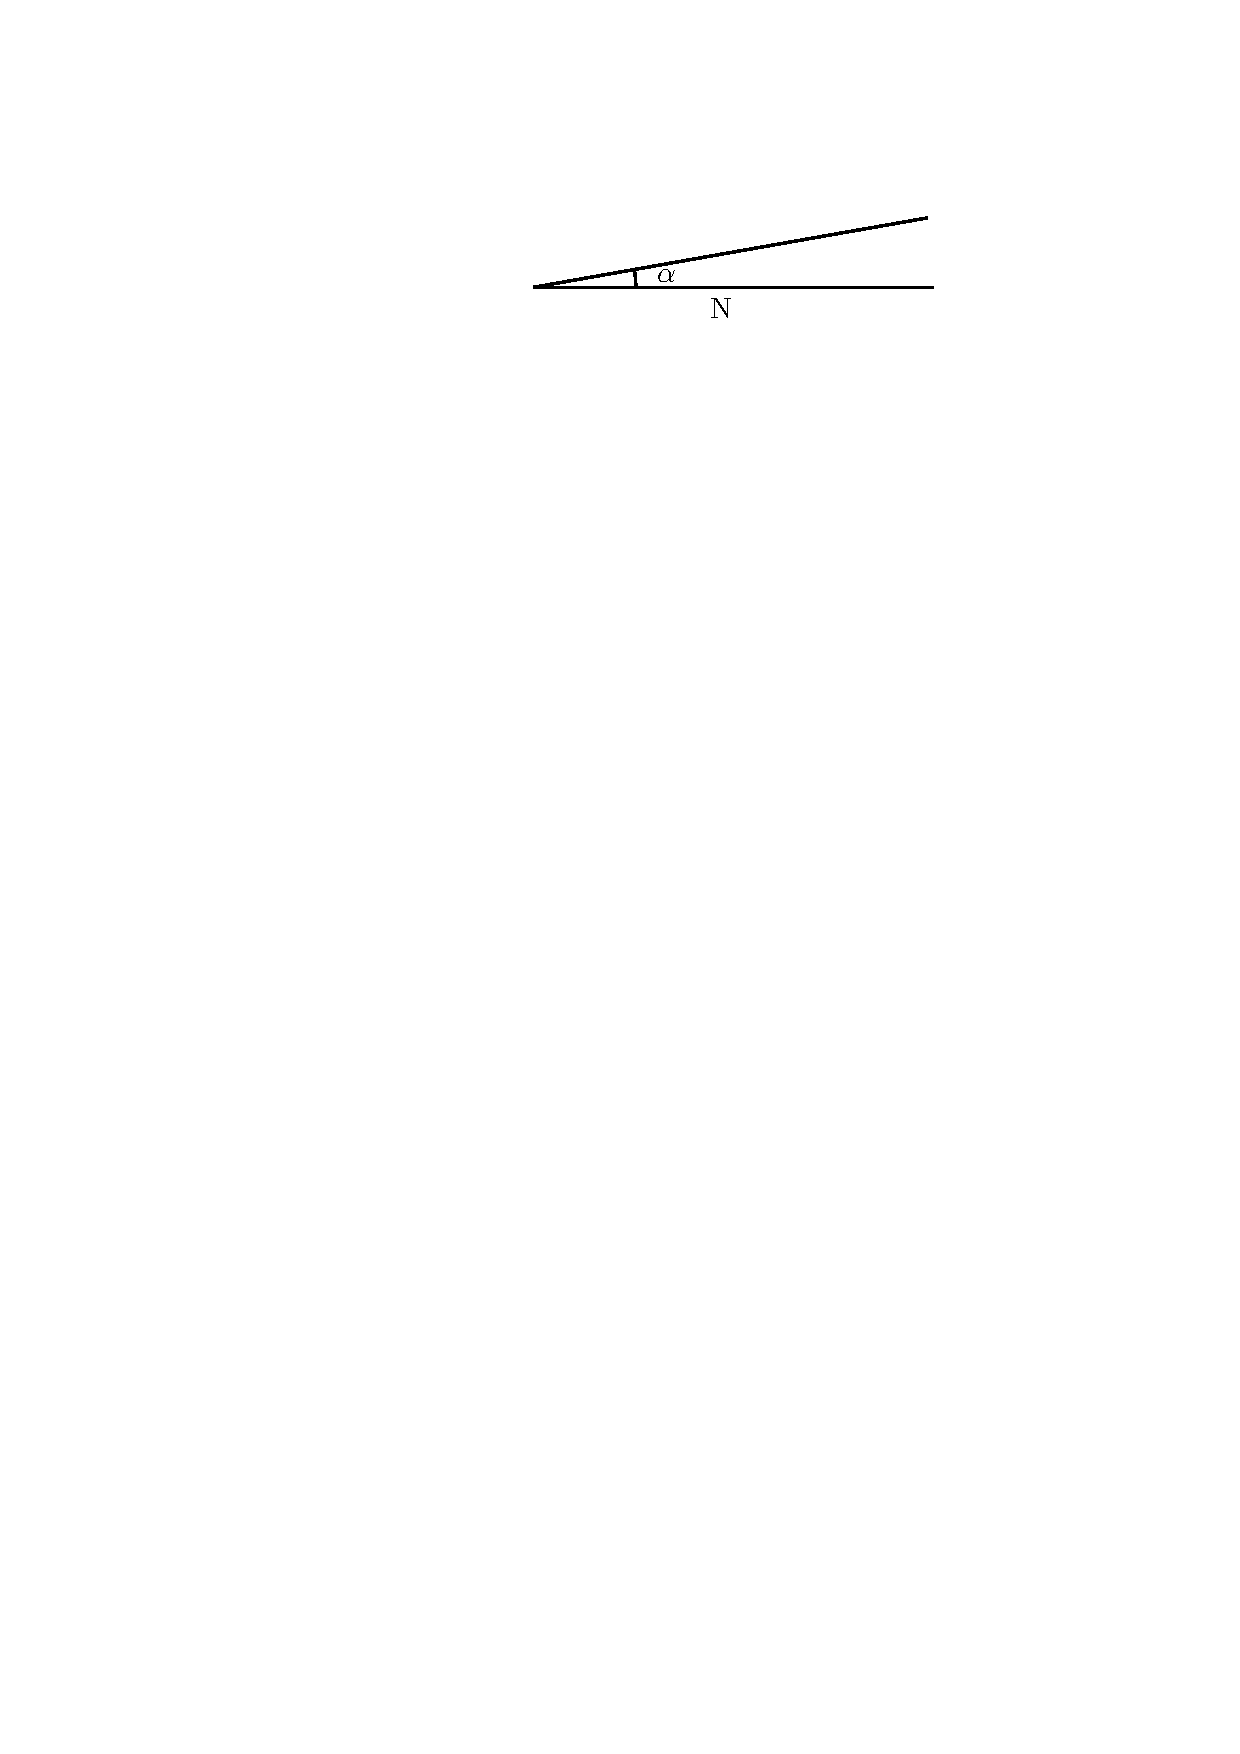
\includegraphics[width=0.45\columnwidth]{graphics/AngularDisplacement.pdf}
% \end{center}
% \end{minipage}



\end{proof}



%To show that the hinge graph is a forest, we construct a simply connected polygonal linkage $(\PP,H)$ that has a realization with fixed orientation if and only if $\Phi$ is satisfiable.
























































































































































% \subsection{Functionality of the Auxilary Construction and Gadgets}
% %Prove Observation 1
% %Prove Observation 2
% %Prove Observation 3
% %Prove Lemma 2
% %Prove Lemma 3 - same as lemma 2 but with tree
% %
% We have described the auxiliary construction.  

% Since the height of the corridor is $\sqrt{3}$, each hexagon has exactly two possible realizations: it can lie either \emph{left} or \emph{right} of the hinge in a horizontal corridor. 
% For simplicity, we use the same notation (R and L) in nonhorizontal corridors, too. 
% Hence, the \emph{state} of each flag in a realization is either L or R. The following observation describes the key mechanism of a corridor.

% \begin{observation}\label{obs:corridor}
% \begin{itemize}
% \item[(1)] If the leftmost hexagon is in state R, then all $t$ hexagons are in state R, and the rightmost hexagon enters the junction on the right of the corridor.
% \item[(2)] Similarly, if the rightmost hexagon is in state L, then all $t$ hexagons are in state L, and the leftmost hexagon enters the junction on the left of the corridor.
% \end{itemize}
% \end{observation}
% The proof of Obesrvation \ref{obs:junction} is as follows:
% \begin{proof}\label{proof:junction}
% PROOF GOES HERE
% \end{proof}

% Prove that all flexagons around a variable gadget are either clockwise or counterclockwise


% Prove that 

% The following lemma summarizes our result about the auxiliary construction.
% \begin{lem}\label{lem:aux}
% For every instance $\Phi$ of P3SAT, the above polygonal linkage with flexible and obstacle polygons has the following properties: (1) it has polynomial size; (2) its hinge graph is a forest;
% (3) it admits a realization such that the obstacle polygons remain fixed if and only if $\Phi$ is satisfiable.
% \end{lem}
% \begin{proof}

% Suppose we have an instance $\Phi$ of P3SAT with $m$ variables and $n$ clauses with a corresponding associated graph $A(\Phi)=(V,E)$ and it is satisfiable.  
% We need to show the following three properties about its corresponding auxilliary construnction: it has polynomial size, its hinge graph is a forest, and it admits a realization such that the obstacle polygons remain fixed.

% \noindent (1) We can bound the number of obstacle hexagons to represent a variable gadget by $2 D$, where $D = \lr{ \max_{v \in V} \deg (v)}$.  
% The number of clause junctions is $n$.
% To give an upper bound on the number of flags in the auxiliary construction, we have to account for the flags in the transmitter gadgets, the extra hexagons found in junctions, and the flags around the variable gadgets.

% Recall that that the number of flags in a corridor are $ t = 2N(m,n)^3 + 1 $ where $N(m,n)$ is a polynomial. 
% Recall that the drawing of $A(\Phi)$ have edges drawn in vertically and horizontally and can join at some ``elbow''.  
% The distance can be measured in the $\ell_1$ norm.
% Similarly in the honeycomb construction, the flexable hexagons zig-zig vertically and horizontally through out honeycomb.  
% The number of corridors about an obstacle hexagon is $6$.
% To give a generous upper bound on the number of flags in a transmitter gadget, is $6 \cdot t \cdot \ell_1\lr{v_i,C_j}$, assuming each obstacle hexagon is of unit height.

% The number of junctions in the auxiliary construction is the number of junctions to form all variable gadgets, transmitter gadgets, and clause gadgets. 
% We know there are at most $2 \cdot D$ obstacle hexagons to form each variable gadget and $6$ junctions for each obstacle hexagon.  
% Therefore an upper bound for the number of flags around variable gadgets is $m \cdot 6 \cdot t \cdot 2 \cdot D$.
% The upper bound for the number of junctions in a transmitter gadget is $6 \ell_1 \lr{v_i, C_j}$.  
% Thus, the upper bound of all junctions in all transmitter gadgets is $$6 \cdot \sum_{\left\lbrace v_i, C_j \right\rbrace \in E} \ell_1 \lr{v_i, C_j}.$$
% The upper bound on the total number of flags is
% $$m \cdot 6 \cdot t \cdot 2 \cdot D + 6 \cdot \sum_{\left\lbrace v_i, C_j \right\rbrace \in E} \ell_1 \lr{v_i, C_j}.$$

% \noindent (2) Recall that a forest is a disjoint union of trees. 
% By construction, each flag is hinged to exactly one obstacle hexagon.  
% There are no hinges between obstacle hexagons.
% Consequently, each component of the hinge graph is a star, where the center corresponds to an obstacle hexagon and the leafs corresponds to the flexable hexagons attached to it.

% \noindent (3) 

% To show that the hinge graph is a forest, we construct a simply connected polygonal linkage $(\PP,H)$ that has a realization with fixed orientation if and only if $\Phi$ is satisfiable.
% We modify the auxiliary construction allowing all polygons to move freely, and by adding extra polygons and hinges so that the hinge graph becomes a \emph{tree}, and the size of the construction remains polynomial. 
% Recall that our auxiliary construction is based on a polynomial section of the hexagonal grid, using obstacle hexagons of side lengths $(5t-1)/2$, unit hexagons (of side length 1), and small hexagons of side length $\frac{1}{3}$. 
% We modify it in 3 steps as follows.

% \begin{enumerate}
% \item Move the obstacle hexagons apart such that the width of each corridor increases from $\sqrt{3}$ to $\sqrt{3}+1/(100N)$.
% \item Replace the unit segment in each the clause gadget by a skinny rhombus of diameter $1.1$ and width $1/(200N)$.
% \item Consider a large (polynomial-size) regular hexagon $R$ that contains all gadgets in our construction, and enclose $R$ by a \emph{frame} of 6 congruent regular hexagons, as shown in Fig.~\ref{fig:frame}(a), hinged together in a path.
% \item Connect the frame and the obstacles in $R$ into a simply connected polygonal linkage: In each obstacle hexagon, the bottom or bottom-left side is adjacent to the frame or to a corridor. Introduce a hinge at the midpoint of one such side in each obstacle hexagon. If this side is adjacent to the frame, then attach the hinge to the frame. Otherwise, the hinge is attached to a new \emph{connector} polygon: a skinny rhombus of diameter 1 and width $1/(200N)$. The far corner of each rhombus is hinged to the unit hexagon in the middle of the corridor at shown in Fig.~\ref{fig:frame}(b).
% \end{enumerate}

% \begin{figure}[htbp]
% 	\centering
% 	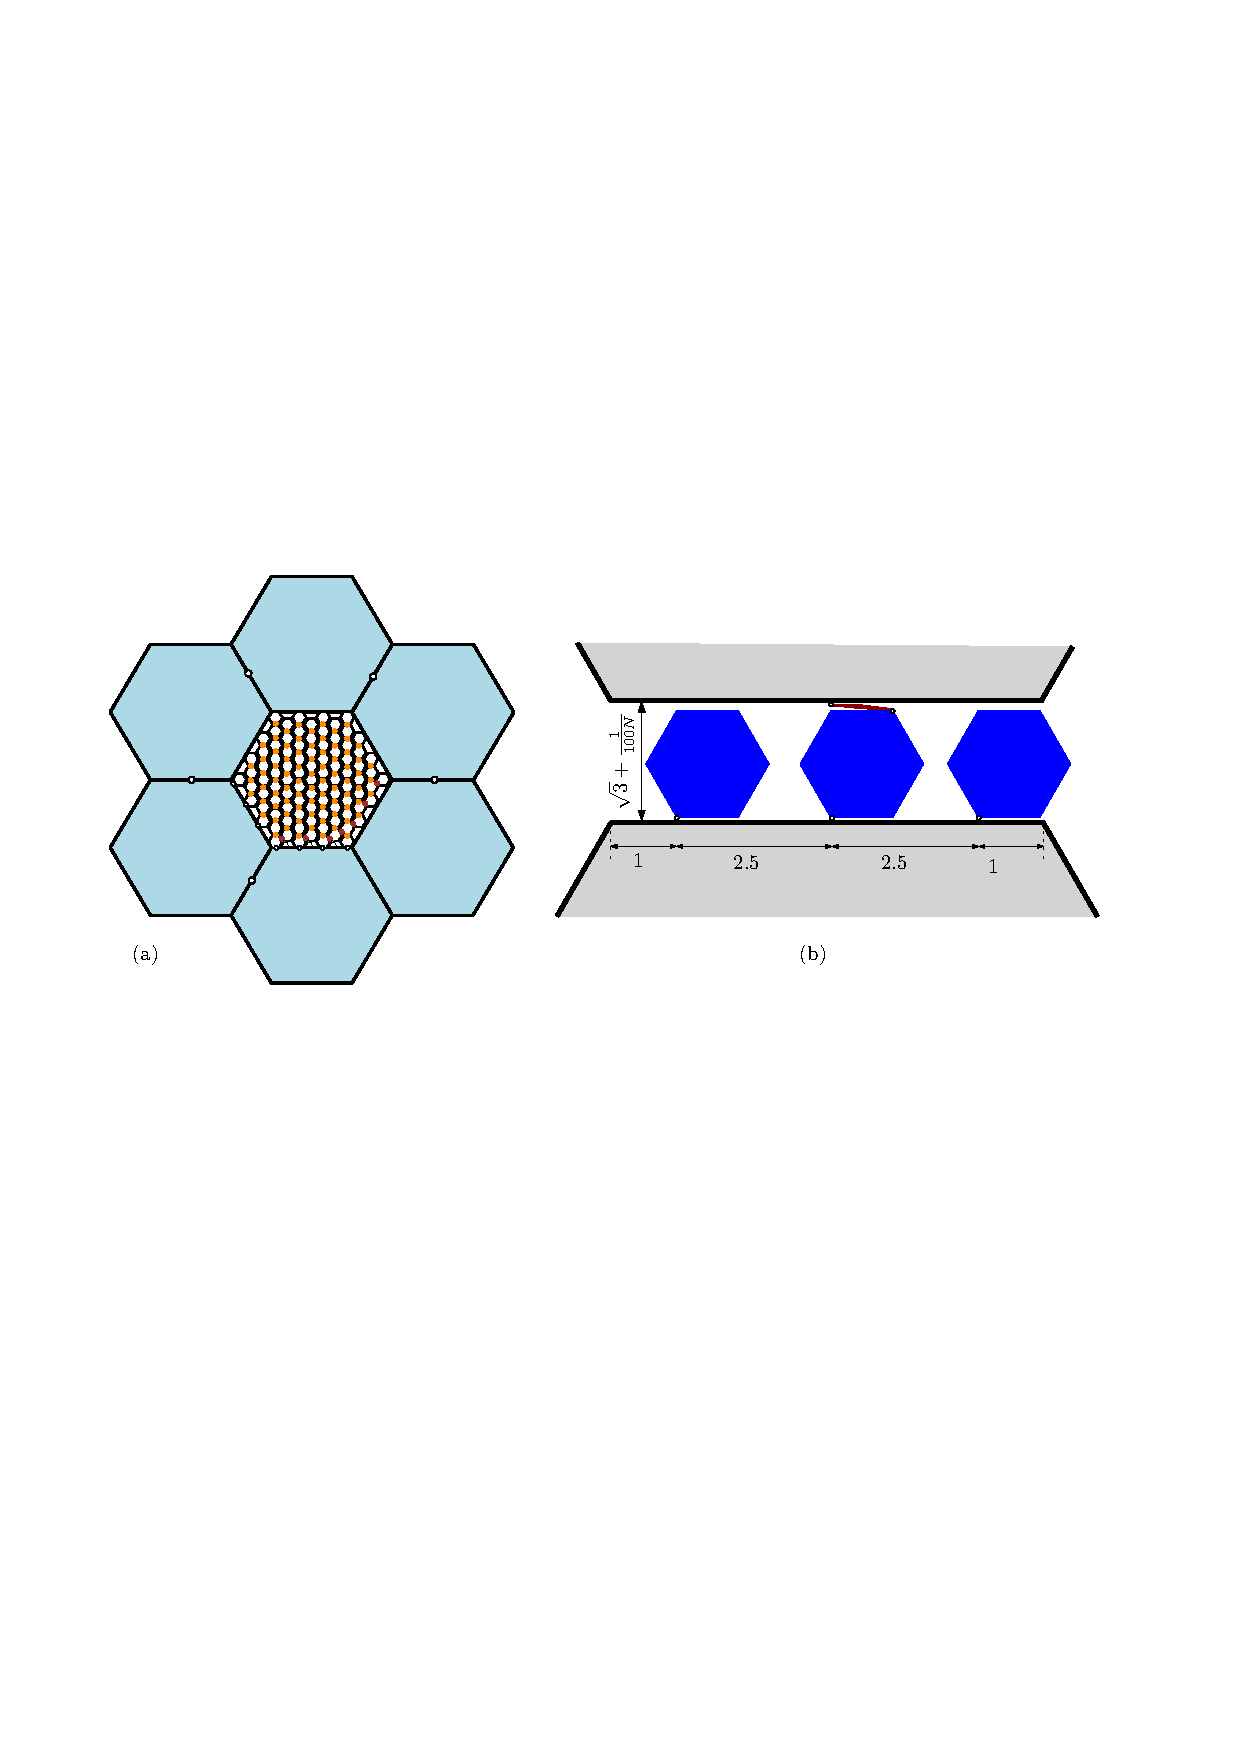
\includegraphics[width=0.95\columnwidth]{graphics/fig-frame-hex}
% 	\caption{(a) A frame (built of 6 hinged regular hexagons) encloses a hexagonal tiling, and
%     vertical paths connect all obstacle hexagons to the frame.
%     (b) A corridor is widened to $\sqrt{3}+1/N^2$. A connection between
%     two adjacent obstacle hexagons is established via a skinny rhombus.}
% 	\label{fig:frame}
% \end{figure}
% We obtain a simply connected polygonal linkage. 
% We now allow the obstacle hexagons to move freely, and call their original fixed position \emph{canonical}. 
% \noindent (3) We may assume without loss of generality that the frame is at its original position. 
% It is enough to show that the obstacle hexagons are still confined to an $1/N$-neighborhood of their canonical position, then it
% follows that the polygonal linkage is realizable if and only if $\Phi$ is satisfiable.






% %Let $\Phi$ be an instance of P3SAT (i.e., a Boolean formula $\Phi$ in 3-CNF with $n$ variables, $m$ clauses, and a planar graph $A(\Phi)$).



% \end{proof}
% The modification of the auxiliary construction is a tree.  
% Satisfiability is an NP-hard problem \cite{cook1971complexity}.
% Thus, we prove Theorem \ref{thm:hinge2}

% The obstacle hexagons in the bottom and bottom-left rows are hinged directly to the frame,
% and so they are locked in their canonical position. Consider two obstacle hexagons on opposite
% sides of a corridor with connector. The distance between the midpoints of the opposite sides of
% the corridor is at least $\sqrt{3}$ (due to the unit hexagons in the corridor) and at most
% $1+\sqrt{3}$ (due to the connector polygon). The length of the corridor is much larger,
% $(5t-1)/2=5N^3+2$, so the orientations of the two adjacent obstacles differ by at most $1/2N^3$.
% Consequently, the orientation of \emph{any} obstacle differs from canonical by at most $1/2N^2$.
% Due to the unit hexagons within the horizontal corridors, the length of any vertical segment between
% the opposite sides of a horizontal corridor is at least $1-1/N^2$. The vertical distance between the
% bottom and top sides of the frame gives an upper bound of  $2N/(100N^2)=1/(50N)$ for the sum of these
% vertical distances. We conclude that the $y$-coordinates of the obstacles are within $1/(10N)$
% of the canonical position. Due to the connector polygons, the $x$-coordinates of
% two adjacent obstacles differ by either less than the vertical offset or by about
% one unit. However, the horizontal distance between the left and right frames prevent
% a shift of this magnitude. So the $x$-coordinates of the obstacle hexagons are also
% within $1/N$ of the canonical position.

